\subsection{Strip Tracker Calibrations}

The silicon strip tracker (SST) of the CMS experiment is the largest detector of its kind in the world, with an active area of 200 $m^{2}$ of silicon \cite{Karimaki:368412,CMS:2000eqx,CMSTrackerGroup:2020edz}.\\
The SST detects charge deposits (hits) at discrete points along the paths of charged particles arising from the collisions produced by the LHC. These hits, together with those detected in the CMS pixel detector (described in Section \ref{sec:PixelCalib}), are used to reconstruct the trajectories of charged particles traversing the detector, thus the SiStrip detector plays a critical role in the High-Level Trigger (HLT) decision-making process.\\
The calibration of its parameters, particularly for tracking and reconstruction, is vital for maintaining performance and ensuring robust data acquisition. This section summarizes the key prospects and current practices for optimizing SiStrip calibrations at HLT.\newline \newline
This part of the report delves into the calibration prospects of the SiStrip detector.\\
Out of the 326 conditions in the HLT GT, 24 are related to the Silicon Strip Tracker, of which 21 are relevant to Run 3 data-taking. 

\begin{table}[h!]
    \centering
    \begin{adjustbox}{max width=\textwidth}
    \begin{tabular}{p{3.4cm}|p{4.6cm}|p{2.5cm}|p{2.5cm}|p{3.5cm}}
        \textbf{Name} & \textbf{Record} & \textbf{Workflow} & \textbf{Frequency of Updates} & \textbf{Description} \\ \hline
      Particle Gain              & \texttt{\textbf{SiStripApvGain2Rcd}}             &   PCL + MRH, manual upload              & Every couple of weeks/couple of months  & Per APV cluster charge calibration  \\ \hline
      Tickmark Gain              & \texttt{\textbf{SiStripApvGainRcd}}              &   O2O                                   & Every couple of weeks/month             & Per APV cluster charge calibration  \\ \hline
      FED cabling                & \texttt{SiStripFedCablingRcd}           &   O2O                                   & Every couple of weeks/month             & Readout to Detector ID mapping  \\ \hline
      Latency                    & \texttt{SiStripLatencyRcd}              &   O2O                                   & Every couple of weeks/month             & Readout algorithm type  \\ \hline     
      Noises                     & \texttt{SiStripNoisesRcd}               &   O2O                                   & Every couple of weeks/month             & Per strip noise  \\ \hline
      Pedestals                  & \texttt{SiStripPedestalsRcd}            &   O2O                                   & Every couple of weeks/month             & Per strip pedestals  \\ \hline
      FED thresholds             & \texttt{SiStripThresholdRcd}            &   O2O                                   & Every couple of weeks/month             & FED cluster finding thresholds  \\ \hline
      Online Bad Strips          & \texttt{SiStripBadStripRcd}             &   O2O                                   & no update                               & Dead strips  \\ \hline  
      Online Bad Modules         & \texttt{SiStripBadModuleRcd}            &   Manual                                & Might be used occasionaly depending on online failures & Dead Modules  \\ \hline   
      Backplane Correction       & \parbox[t]{5cm}{\texttt{SiStripBackPlaneCorrectionRcd,}\\\texttt{deconvolution}}  &   Manual                   & no update                               & Cluster position corrections  \\ \hline      
      Backplane Correction       & \parbox[t]{5cm}{\texttt{SiStripBackPlaneCorrectionRcd,}\\\texttt{peak}}           &   Manual                   & no update                               & Cluster position corrections   \\ \hline          
      Online Bad Channels        & \texttt{SiStripBadChannelRcd}           &   Manual                                & no update                               & Dead channels  \\ \hline                                      
      Online Bad Fibers          & \texttt{SiStripBadFiberRcd}             &   Manual                                & no update                               & Dead fibers  \\ \hline                                        
      Cluster finding thresholds & \texttt{SiStripClusterThresholdRcd}     &   Manual                                & no update                               & Cluster finding thresholds   \\ \hline
      Online Configuration       & \texttt{SiStripConfObjectRcd}           &   Manual                                & no update                               &    \\ \hline                            
      Online Configuration       & \parbox[t]{5cm}{\texttt{SiStripConfObjectRcd,}\\\texttt{apvphaseoffset}}  &   Manual   & no update                               &  \\ \hline
      Dead channels              & \texttt{SiStripDetVOffRcd}              &   Manual                                & no update                               & List of Unpowered modules  \\ \hline
      Lorentz Angle              & \parbox[t]{5cm}{\texttt{SiStripLorentzAngleRcd,}\\\texttt{deconvolution}} &   Manual & no update & Hall mobility per unit magnetic field  \\ \hline
      Lorentz Angle              & \parbox[t]{5cm}{\texttt{SiStripLorentzAngleRcd,}\\\texttt{deconvolution}} &   Manual & no update & Hall mobility per unit magnetic field  \\
    \end{tabular}
    \end{adjustbox}
    \caption{Fundamental SiStrip Calibrations, ordered in terms of frequency of updates.}
    \label{tab:StripCalibrations_critical}
\end{table}

\subsubsection{Hit Reconstruction in the Strip Detector}

The data acquisition system (DAQ) of the strip detector processes signals through algorithms executed on off-detector electronics, specifically on the front-end driver (FED) modules~\cite{CMS:2014pgm}. These algorithms:
\begin{itemize}
    \item Subtract pedestals (baseline signal levels without particles).
    \item Remove common mode noise (event-by-event baseline fluctuations within each tracker chip).
    \item Perform zero-suppression, retaining only strips with charges exceeding specific thresholds:
    \begin{itemize}
        \item \(> 5\sigma\) above the channel noise, or
        \item \(> 2\sigma\) for a strip and at least one neighbor.
    \end{itemize}
\end{itemize}

As a result, only a fraction of channels are stored offline for further processing.\\

Offline, clusters are formed by:
\begin{enumerate}
    \item Seeding with strips that pass zero-suppression and have charges \(> 3\sigma\) above the noise.
    \item Adding neighboring strips with charges \(> 2\sigma\).
    \item Retaining clusters with total charge \(> 5\sigma_{\text{cluster}}\), where:
    \[
    \sigma_{\text{cluster}} = \sqrt{\sum_i \sigma_i^2},
    \]
    and \(\sigma_i\) is the noise for strip \(i\).
\end{enumerate}

The position of each hit is determined as the charge-weighted average of strip positions, corrected for:
\begin{itemize}
    \item Lorentz drift, shifting hits by approximately \(10~\mu\text{m}\) in the Tracker Inner Barrel (TIB) and \(20~\mu\text{m}\) in the Tracker Outer Barrel (TOB).
    \item Inefficient charge collection near the sensor backplane, introducing a \(10~\mu\text{m}\) shift in 500~\(\mu\text{m}\) thick silicon, but negligible in 320~\(\mu\text{m}\) thick silicon.
\end{itemize}

The inefficiency arises from the narrow time window of the APV25 readout chip, which limits charge integration and reduces out-of-time background.\\

The hit position uncertainty is usually parametrized based on the expected cluster width from the track angle. However:
\begin{itemize}
    \item For clusters with observed widths exceeding the expected width by \(> 3.5\times\), the uncertainty is set to the binary resolution:
    \[
    \text{Binary Resolution} = \frac{\text{Cluster Width}}{\sqrt{12}}.
    \]
    \item This broadening is caused by capacitive coupling between strips or energetic delta rays.
\end{itemize}

\subsubsection{DAQ O2O Conditions}
The Strip Data Acquisition (DAQ) \emph{Offline-to-Online} (O2O) (discussed in Section \ref{sec:CMScalibration}) populates tracker conditions from the online master data storage (\texttt{OMDS}) to the offline reconstruction conditions database (\texttt{ORCON}). 
Six types of payloads are populated in this O2O: 
\begin{itemize}
\item \texttt{SiStripBadStrip} 	
\item \texttt{SiStripFedCabling} 	
\item \texttt{SiStripLatency} 	
\item \texttt{SiStripNoises} 	
\item \texttt{SiStripPedestals} 	
\item \texttt{SiStripThreshold}
\end{itemize}

These records hold conditions including information about the detector's configuration during data-taking, such as cabling, module connections, and control parameters. The O2O framework facilitates the synchronization of online settings with offline processing, enabling accurate interpretation of the data. This ensures that the conditions under which the detector operated, including potential changes in configuration or performance during data-taking, are faithfully reproduced in offline analyses, maintaining the integrity and quality of the physics results.

\subsubsection{DCS O2O Conditions}
The record \texttt{SiStripDetVOffRcd} is designed to hold information coming from the Strip Detector Control System (DCS) O2O (discussed in Section \ref{sec:CMScalibration}).\\ This workflow populates the Strip tracker High Voltage (HV) / Low Voltage (LV) information from PVSS online database to the offline condition database (\texttt{ORCON}, see Fig.~\ref{fig:CondDB}). The DCS information is used in prompt reconstruction but currently not in the HLT, thus the payload used in the HLT reconstruction is empty (all channels are marked as fully powered).\\
Modules that are OFF are retrieved form the PVSS database and stored in the condition database via hourly cron jobs. Three cron jobs are set up for the DCS O2O, including one production job and two validation jobs, each write to a different tag in the condition database with a different delay in time: 
\begin{itemize}
\item 1 hour Delay Validation: populates HV/LV states until 1 hour before the cron job execution;
\item 13 hours Delay Validation: populates HV/LV states until 13 hour before the cron job execution;
\item 25 hours Delay Validation: populates HV/LV states until 25 hours before the cron job execution. Also synchronized to the tag used in production for prompt reconstruction;
\end{itemize}

\subsubsection{Bad Components}
For the identification of bad components dedicated to a given run it is important that the analysis is based on data which do not take into account the knowledge of bad components identified during the offline analysis of previous runs.\\
This has to be ensured because bad components might be recovered from one run to another so that they have to be qualified unbiased afterwards. Since the reconstruction chain used to produce the usual tracker \texttt{AlCaReco} streams already includes bad components from offline analysis, these streams cannot be used here.

Therefore, a \texttt{AlCaReco} (see Section~\ref{sec:CMScalibration}) stream dedicated to the bad component identification in the strip tracker was introduced in the \texttt{AlCaReco} workflow. It is called \texttt{ALCARECOSiStripCalZeroBias} and has the following properties:
\begin{itemize}
\item  The input is the digitized output from standard reconstruction since it is independent from bad channel masking. The reconstruction is performed up to cluster (so only the digi to cluster step is performed in the \texttt{AlCaReco}).
\item Only bad components from cabling and O2O are taken into account during reconstruction. Bad components from offline analysis are not considered.
\item Only events with random trigger are selected. For collision data the HLT path \texttt{HLT\_ZeroBias} and for cosmic data the \texttt{HLT\_Random} is chosen.
\item The output of the stream contains only the cluster collection and the \texttt{L1AcceptBunchCrossings} collection (needed by the filters against the APV25 readout chip \cite{French:2001xb} induced noise). This can be used as starting point in case the calibration has to be redone.
\item The DQM output contains one cluster occupancy histogram per strip detector. These histograms are used as input for the bad component algorithms. In addition, the \texttt{ClusterVsAPVCycle} and the \texttt{TotalNumberOfCluster} histograms are stored for each subdetector. 
\end{itemize}

Once the DQM output of a given run with enough statistics is available from the central DQM harvesting, the bad component identification can be performed.\\ Fig.~\ref{fig:fill10200PCL_0} shows schematically the workflow for the Strip bad components identification.

\begin{figure}[htbp]
   \centering
	\includegraphics[width=0.7\textwidth]{figures/BadComponentWorkflow_small.png}
   \caption{The workflow for the Strip Bad Component Identification is shown in the sketch above.}
   \label{fig:fill10200PCL_0}
\end{figure}

\subsubsection{APV Gains}
The total charge of a strip cluster in the CMS detector is calculated by summing the contributions from each individual strip in the cluster. For each strip, the raw ADC counts are corrected using two gain factors, \(\text{G1}_i\) and \(\text{G2}_i\), which are specific to the strip. The charge for the entire cluster is then obtained by the following formula:

\[
Q_{\text{cluster}} = \sum_{i=1}^{N} \frac{\text{ADC}_i}{\text{G1}_i \times \text{G2}_i}
\]

Where:
\begin{itemize}
    \item \( Q_{\text{cluster}} \) is the total charge of the cluster.
    \item \( N \) is the number of strips in the cluster.
    \item \( \text{ADC}_i \) is the ADC count for the \( i \)-th strip.
    \item \( \text{G1}_i \) is the first gain factor for the \( i \)-th strip.
    \item \( \text{G2}_i \) is the second gain factor for the \( i \)-th strip.
\end{itemize}

The ADC count for each strip represents the raw signal from the detector. The gain factors \(\text{G1}_i\) and \(\text{G2}_i\) are applied to convert the ADC counts into the corresponding physical charge. These gains may vary across strips due to differences in calibration and detector characteristics.
The gain calibration is performed in two sequential steps, each one delivering a
calibration factor. These steps, referred as the calibration sequence, are:

\begin{itemize}
\item Tick Mark calibration (\texttt{SiStripApvGainRcd}) (so called G1): the tick marks are external signals, input into the readout chips every 35 LHC clocks, that are used to synchronize the tracker modules to the central trigger.
When the detector is synchronized, the height of the voltage pulse at the tick mark is equalized in gain among all the readout chips to 640 ADC counts. This calibration corrects for the electronic effects at the readout level but does not account for the differences at the sensor level.\\
This is performed via the so-called tickmark O2O 
\item Particle Calibration (\texttt{SiStripApvGain2Rcd}) (so called G2): the particle calibration equalizes the detector response for the measurement of minimum ionizing particles (m.i.p.) charge. \\
The charge measured by each cluster on track is corrected for the track path in the sensor depletion region and therefore used to build the distribution of the ionization charge per unit of length. The voltage gain is tuned to have the most probable value of these distributions, made for every sensors, set to 300 ADC counts / mm. This procedure requires a lot of track statistics (around 1B clusters).\\
This is performed via a multi-run harvesting based PCL workflow.
\end{itemize}

Fig.~\ref{fig:StripClusterCharge} shows the time evolution of the calibrated SiStrip cluster charge (after having applied both the tickmark and particle level gain calibraitons) as a function of the integrated luminosity during LHC Run 3. 
 
\begin{figure}[htbp]
   \centering
	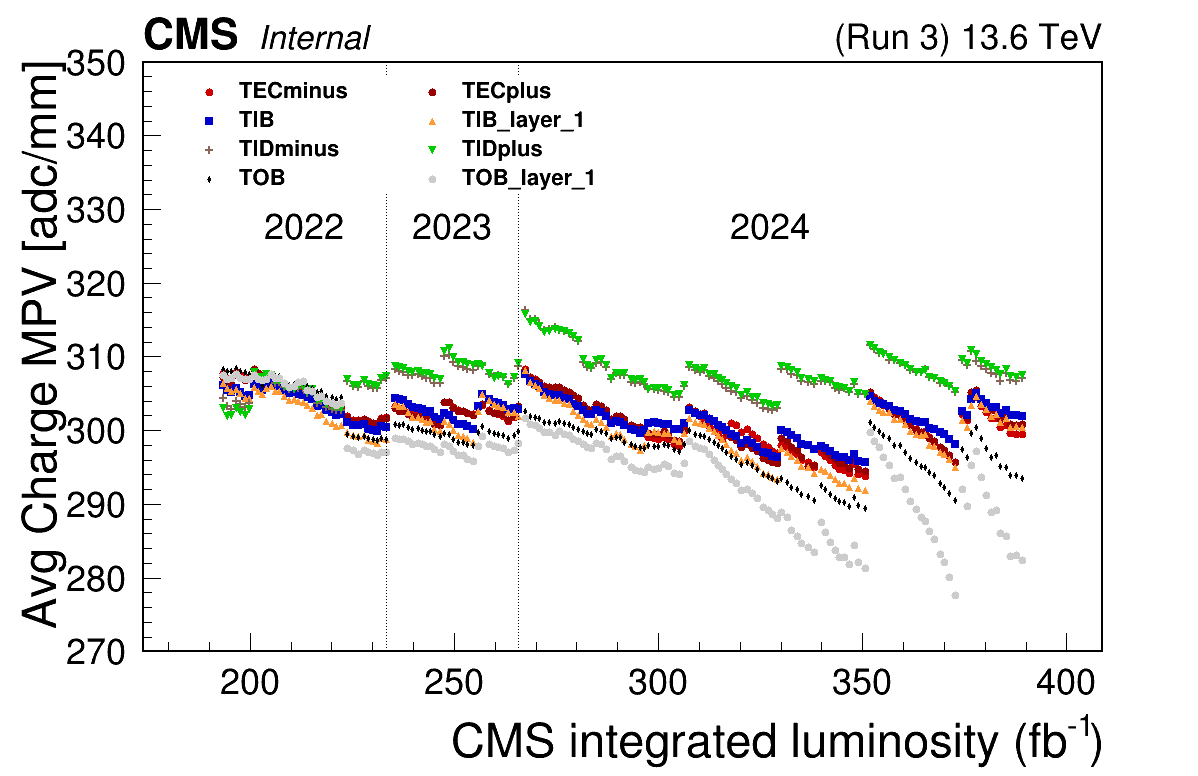
\includegraphics[width=0.8\textwidth]{figures/CalibratedCharge_run3_lumi.png}
   \caption{Time evolution of the calibrated SiStrip cluster charge as a function of the integrated luminosity during LHC Run 3, shown separately for different detector regions. Discontinuities in the trends correspond to periodic re-calibrations. The increasing deviations from the nominal calibration value of 300 ADC/mm highlight the impact of silicon sensor and readout fiber ageing, emphasizing the need for more frequent calibration updates to maintain optimal detector performance.}
   \label{fig:StripClusterCharge}
\end{figure}

\subsubsection{CPE Conditions}

\begin{itemize}
    \item Two key CPE-related conditions are maintained:\newline
    \texttt{SiStripLorentzAngleRcd} and \texttt{SiStripBackPlaneCorrectionRcd}.
    \item Both conditions are provided in two configurations: "deconvolution" and "peak," depending on the readout mode.
    \item Updates to these calibrations require dedicated workflows involving special datasets (e.g., cosmics, low pile-up collisions).
    \item The conditions have seen minimal updates since early Run 2, as miscalibrations are often treated as geometric mispositioning during tracker alignment procedures.
    \item A monitoring workflow exists in the Prompt Calibration Loop (PCL), but direct calibration at HLT is limited.
\end{itemize}

\subsubsection{NGT Demonstrator Candidate Evaluation}

To summarise the main NGT calibration workflow candidates:
\begin{itemize}
    \item \textbf{Bad Components Masking}:
    \begin{itemize}
        \item Already implemented in PCL workflows and requires minimal statistics for updates.
        \item Demonstrated to improve track building in inside-out muon reconstruction.
    \end{itemize}
    \item \textbf{Particle Gains Calibration (a.k.a. G2)}:
    \begin{itemize}
        \item High-statistics requirement makes frequent updates infeasible.
        \item Potential minor impact on track building and cluster charge thresholds.
    \end{itemize}
\end{itemize}

The recommendations in the context of the NGT calibration workflow are:
\begin{itemize}
    \item Prioritize the inclusion of bad components masking in the NGT demonstrator workflow due to its operational simplicity and demonstrated impact.
    \item Consider periodic evaluations for integrating gain calibrations as part of long-term upgrades.
\end{itemize}